%% This is a skeleton file demonstrating the use of IEEEtran.cls (requires IEEEtran.cls version 1.8a or later) with an IEEE conference paper.
%%
%% Modified by Khan Reaz( kahn.reaz@ieee.org)
%% Support sites:
%% http://www.ieee.org/

%%***********************************************************
%% Legal Notice:
%% This code is offered as-is without any warranty either expressed or implied; without even the implied warranty of MERCHANTABILITY or FITNESS FOR A PARTICULAR PURPOSE!
%% User assumes all risk and can modify as s/he wants.

%%***********************************************************

\def\b0{{\bf 0}}
\def\ba{{\bf a}}
\def\bb{{\bf b}}
\def\bc{{\bf c}}
\def\bd{{\bf d}}
\def\be{{\bf e}}
\def\bg{{\bf g}}
\def\bh{{\bf h}}
\def\bi{{\bf i}}
\def\bj{{\bf j}}
\def\bk{{\bf k}}
\def\bl{{\bf l}}
\def\bm{{\bf m}}
\def\bn{{\bf n}}
\def\bo{{\bf o}}
\def\bp{{\bf p}}
\def\bq{{\bf q}}
\def\br{{\bf r}}
\def\bs{{\bf s}}
\def\bt{{\bf t}}
\def\bu{{\bf u}}
\def\bv{{\bf v}}
\def\bw{{\bf w}}
\def\bx{{\bf x}}
\def\by{{\bf y}}
\def\bz{{\bf z}}


\def\bSigma{{\bf \Sigma}}
\def\bA{{\bf A}}
\def\bB{{\bf B}}
\def\bC{{\bf C}}
\def\bD{{\bf D}}
\def\bE{{\bf E}}
\def\bF{{\bf F}}
\def\bG{{\bf G}}
\def\bH{{\bf H}}
\def\bI{{\bf I}}
\def\bJ{{\bf J}}
\def\bK{{\bf K}}
\def\bL{{\bf L}}
\def\bM{{\bf M}}
\def\bN{{\bf N}}
\def\bO{{\bf O}}
\def\bP{{\bf P}}
\def\bQ{{\bf Q}}
\def\bR{{\bf R}}
\def\bS{{\bf S}}
\def\bT{{\bf T}}
\def\bU{{\bf U}}
\def\bV{{\bf V}}
\def\bW{{\bf W}}
\def\bX{{\bf X}}
\def\bY{{\bf Y}}
\def\bZ{{\bf Z}}


%package list
\documentclass[conference]{IEEEtran}
\IEEEoverridecommandlockouts
\let\labelindent\relax
% \usepackage{breqn}
\usepackage{enumitem}
\usepackage{fleqn}
\usepackage{cite}
\usepackage{graphicx}
\usepackage[varg]{newtxmath}
\graphicspath{ {images/} }
\usepackage{pdfpages}
\usepackage{wrapfig}
\usepackage{fancyhdr}
\usepackage{lastpage}
\usepackage{lettrine}
\usepackage{amsmath}
% \usepackage{titlesec}
\usepackage[colorinlistoftodos]{todonotes}
\usepackage{float}
\usepackage[font={footnotesize}]{caption}
\usepackage[numbers,sort,square,compress]{natbib}
\usepackage[para]{footmisc}
\usepackage{xcolor}
\setlength{\belowcaptionskip}{-12pt}
\newcommand{\highlight}[1]{%
  \colorbox{red!50}{$\displaystyle#1$}}

% \usepackage{parskip}
% \setlength{\parskip}{0.02\baselineskip}

% \fancypagestyle{plain}{
%   \fancyhf{} % sets both header and footer to nothing
% \renewcommand{\headrulewidth}{0pt}
%   \fancyhead[C]{2018 International Conference on Indoor Positioning and Indoor Navigation (IPIN), 24-27 September 2018, Nantes, France}% Right header

% }
\pagestyle{plain}% Set page style to plain.

% \pagestyle{fancyplain}
% \fancyhf{}
% \renewcommand{\headrulewidth}{0pt}
% \fancyhead[C]{2018 International Conference on Indoor Positioning and Indoor Navigation (IPIN), 24-27 September 2018, Nantes, France}
\DeclareMathOperator*{\argmin}{argmin}
% \usepackage{titlesec}

% \titlespacing*{\section}{0pt}{1pt plus 2p}{1ex}
% \titleformat*{\section}{\fontsize{12}{12}\bfseries}
% \titleformat{\section}
%        {\normalfont\fontfamily{phv}\fontsize{12}{17}\bfseries}{\thesection}{1em}{}

% \titleformat{\subsection}
%        {\normalfont\fontfamily{phv}\fontsize{12}{17}\bfseries\itshape}{\thesubsection}{1em}{}

\begin{document}
%Here goes the title

\title{Scalar Parametrization for Joint Time-Frequency interpolation in a MIMO-OFDM channel}


%Authors List

 \author{\authorblockN{Author 1, Author 2, Author 3}
 \
 \authorblockA{Department of Electrical Engineering, Indian Institute of Technology Bombay}
% \thanks{Parts of this work was supported by the Bharti Centre for Communication in
% IIT Bombay, and the Visvesvaraya
% PhD Scheme of Ministry of Electronics \& Information Technology,
% Government of India (implemented by the Digital India Corporation).
% }}
}
\maketitle

\thispagestyle{plain}
%Main body starts



% \noindent We consider problem of quantization and interpolation of
% time and frequency varying precoding matrices in wireless MIMO
\begin{abstract}
In a limited feedback MIMO channel, the performance of the channel can improve significantly if the transmitter knows the channel state information(CSI). The receiver knows the channel information, and it feeds back to the transmitter. However, it is not possible to feedback complete information for a limited-feedback OFDM channel since the channel information for multiple subcarriers consumes a large amount of data. Therefore to resolve this problem, the orthonormality structure of the precoder matrix is exploited to make its one-to-one mapping to a minimal number of scalar parameters. The Precoder matrix is decomposed using Givens Rotation. For an i.i.d. flat-fading Rayleigh channel, these parameters are independent, which makes its quantization and interpolation easy. We propose an efficient method for quantization of the channel state information at the receiver by using adaptive delta modulation for successive time interval. We also propose a method for joint time-frequency interpolation of the channel information at the transmitter. 153-words
\end{abstract}

\section{Introduction}
\label{intro}

% no need to write the numbers in your introduction. You start by explaining what is happenning currently and then propose your solution.
The use of multiple antennas at the transmitter and receiver can significantly enhance the performance of wireless systems. Moreover, in these multiple-input multiple-output (MIMO) wireless systems, the transmitter can perform an better resource allocation if channel state information (CSI) is made available at the transmitter, both to improve data rates and reduce BER~\cite{love2008overview}. To this end, feeding back the channel state information from the receiver to the transmitter efficiently is necessary. In the many wireless systems that use orthogonal frequency division multiplexing (OFDM), the feedback needs to be provided to the transmitter across the many subcarriers of the system, which places a large feedback demand. However, since the channel state information varies gradually in both time and frequency, effective techniques to reduce feedback overheads exist, using frequency interpolation temporal prediction. In this paper, we focus on the problem of tracking the precoders of a MIMO-OFDM system across time and frequency for efficient CSI feedback.

In recent years, codebook design over the Stiefel Manifold \cite{6891198} has been proposed where the manifold structure of the channel matrix is used for its predictive quantization and interpolation across time and frequency. Another such variation of \cite{6891198} has exploited both time and frequency domain together in Stiefel Manifold \cite{Gupt1905:Predictive}. All these methods are useful, but they do so over Manifolds which has problems of getting stuck in local Maxima. Also, there are different challenged which are faced while interpolating in a high dimensional space.

Another very different approach in \cite{4114278} has tried to break down the precoder matrix into independent scalar parameters using transformations, namely Givens rotation and Household Transformation. They are tracking each of these scalar parameters using ADCPM(Adaptive Digital Pulse Code Modulation) for a slowly varying channel in the time domain. They have shown capacity achieved with the quantized precoding matrix to be very close to the unquantized one. In another paper \cite{4556174}, they have exploited frequency and performed ADPM in frequency domain to achieve similar performance with a lower number of feedback bits.

We now propose a method for predictive quantization in time domain over few subcarriers using scalar parameters. We also propose a method for exploiting the joint time-frequency correlation of those scalar parameters on the transmitter side. In \ref{section2}, we start by explaining the system model and the method for scalar quantization \& interpolation of the precoder matrix. In \ref{section3}, we perform various simulations for our approach and show the benefits from the improved BER rates and Achievable Rate.
%Since $H=U\Sigma V$, it is sufficient to quantize V*(precoder) and send this information back. In an OFDM channel, this data consume significant amount of bits and therefore, sending the complete data could consume too much bandwidth data. For e.g. an OFDM channel with 4 transmitters, 2 receiver antennas, and 64 subcarriers would require 64*(no. of bits required to send one precoder ~ 12-16 bits) ~ 896 bits per frame. This information could be significantly reduced if we provide better quantization and interpolation techniques/strategies. Also, the matrices which need to be fed back could be broken down into independent scalar parameters. These scalar quantities could be later quantized and interpolated.
% Broad summary of your work, come to your problem definition.

\section{System Model}
\label{section2}
For a MIMO-OFDM system with $N_T$ transmitter and $N_R$ receiver antennas, each subcarrier $i$ with time instant $t$ could be modelled as a flat-fading MIMO channel. This flat-fading MIMO channel could be modelled as
\vspace{-1pt}
\begin{equation}
y_{i,t} = H_{i,t} x_{i,t}+ \eta
\end{equation}

\vspace{-1pt}
where the channel matrix $H_{i,t} \in \mathbb{C}^{N_R \times N_T}$; the input $x_{i,t} \in \mathbb{C}^{N_T}$; the output $y_{i,t} \in \mathbb{C}^{N_R}$ and $\eta$ is the complex additive white gaussian noise vector with distribution $\tilde{\mathcal{N}}(0,I_{N_R})$. On applying thin SVD to H, we get $H_{i,t} = U_{i,t} \Sigma_{i,t} V_{i,t}^{H}$, where $U_{i,t} \in \mathbb{C}^{N_R \times N_T}$, $\Sigma_{i,t} \in \mathbb{C}^{N_T \times N_T}$  and $V_{i,t} \in \mathbb{C}^{N_T \times N_T}$. $U_{i,t}$ and $V_{i,t}$ are orthonormal column matrices and $\Sigma_{i,t}$ contains the singular values $\sigma_1 \geq \ldots \geq \sigma_{N_T} > 0$ of H. The entries of H are assumed to be i.i.d. $\tilde{\mathcal{N}}(0,1)$, complex circularly symmetric Gaussian with mean zero and variance 1. Therefore, the first n column vectors of $V_{i,t}$ have to be quantized and fed back to the transmitter as channel spatial information.



% Givens rotation definition and how we are decomposing, Theta- pdf = 2lsin(theta)(2l-1).cos(theta) 0 $\leq$ Theta $\leq$ pi/2.
% Householders' transformation and how we are decomposing. -pi$\leq$ phi $\leq$ pi. Uniformly distributed.

% Low-complexity quantization scheme based on a further parameterization of a vector in
% terms of a minimal number of independent scalar parameters. In particular, we consider its application to CSI feedback in slowly time-varying MIMO channels


\subsection{Scalar Paramaterization}
\label{givens}
The degrees of freedom in the spatial information matrix is much smaller than the number of real entries in the matrix because of the geometrical structure between the columns of the matrix \cite{4114278}. An orthonormal matrix with $t$ rows and $n$ columns can be represented as

\begin{equation}
\textbf{V} = \Bigg[\prod_{k=1}^{n} D_{k} \big( \phi_{k,k},\ldots , \phi_{k,n} \big) \: \Bigg\{ \prod_{l=1}^{l=t-k} G_{t-l,t-l+1} \big( \theta_{k,l}\big) \Bigg\} \Bigg] \: \tilde{I}
\end{equation}

where $D_{k}$ is the diagonal matrix given as $D_{k}\big(\phi_{k,k}, \ldots, \phi_{k,t} \big)$ =  $diag\big( 1_{k-1}, e^{j\phi_{k,k}},\ldots, e^{j\phi_{k,t}}  \big)$, $1_{k-1}$ is (k-1) ones; and t x n matrix $\tilde{I}$ = $\big[I_{n}, 0_{n,t-n}\big]^{T}$. The Givens matrix \textbf{G} is given as

\begin{equation}
G_{m-1,m}\big(\theta\big)  =
\begin{bmatrix}
I_{m-2} & & & \\
& cos\;\theta & - sin\;\theta & \\
& sin\;\theta & cos\;\theta & \\
& & & I_{t-m}
\end{bmatrix}
\end{equation}

% \begin{equation}

\begin{figure}
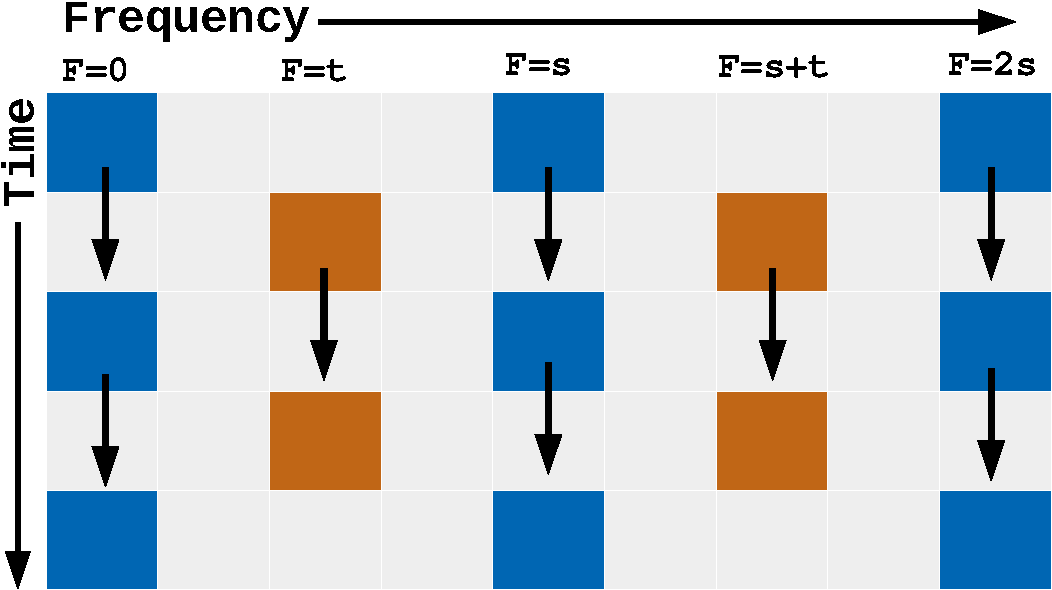
\includegraphics[width=0.5\textwidth]{images/adpm.pdf}

\caption{Subcarriers which need to be quantized}
\label{ber_overvie}
\vspace{-5pt}
\end{figure}

For a $4 \times 2$ orthogonal matrix V,
$$V = D_{1}(\phi_{1,1},\ldots,\phi_{1,4}).G_{3,4}(\theta_{1,1}) .G_{2,3}(\theta_{1,2}) .G_{1,2}(\theta_{1,3})$$
\vspace{-1.4em}
\hspace{1pt}$$.D_{2}(\phi_{2,2},\phi_{2,3},\phi_{2,4}) .G_{3,4}(\theta_{2,1}) .G_{2,3}(\theta_{2,2}).\tilde{I}$$

Here, we denote $\phi_{i}'s$ by phases and $\theta_{i}'s$ by rotation angles. $\phi \in (-\pi, + \pi]$ is uniformaly distributed between the two extremes\cite{4114278}, while $\theta$ has a distribution
\begin{equation}
p(\theta) = 2lsin(\theta)^{2l-1}cos(\theta), \theta \in [0, \frac{\pi}{2}), for \; l = 1,2,\ldots,t-1
\end{equation}
Here all $\theta_i$ and $\phi_i$ are statistically independent which is usefel for tracking them across time as explained in the next subsection. The total number of parameters obtained from the decomposition of a complex orthogonal matrix $N_{T} \times N_{R} $ is given by the relation $N_{R}(2N_{T} - N_{R}) $ \cite{4114278}. Number of $\phi = N_{R}(2N_{T} - N_{R}-1)/2$ while the number of $\theta = N_{T}(2N_{T} - N_{R}+1)/2$
% may cross pi and come immediately to -pi, therefore, values are unwrapped while calculating them. Unwrapping is performed at the receiver over the frequency initially and later in time.
% To exploit the interpolation of time \& frequency jointly at the transmitter, feedback bits are sent in an alternating fashion as shown in the figure.

\subsection{Differential Quantization - Channel Tracking}
\label{quantiz}
For a slowly time varying channel, ADPM is an effective method for tracking a paramater over time with using only 1-bit. The 1-bit number $\beta_{n} = Q(x_{n} - \hat{x}_{n-1})$ where $x$ is the unquantized vector \& $\hat{x}$ is the quantized vector and $Q(x)$ is the quantization function given as

\begin{equation}
  Q(x)=\begin{cases}
    1, & \text{if $x>0$}.\\
    -1, & \text{otherwise}.
  \end{cases}
\end{equation}

Thus, the quantied vector $\hat{x}_n$ changes with time as
\begin{equation}
\hat{x}_{n} = \hat{x}_{n-1} + \beta_{n}\Delta_{n}
\end{equation}
\begin{equation}
\Delta_{n} = \begin{cases}
    M \Delta_{n-1}, & \text{if $\beta_{n} = \beta_{n-1}$}.\\
    \Delta_{n-1}/m , & \text{if $\beta_{n} \neq \beta_{n-1}$}.
  \end{cases}
\end{equation}

Here we initialize delta using $\Delta_1 = abs(x_{2}-\hat{x}_1)$.

We need to quantize the subcarriers in a way such that we can exploit the joint time-frequency interpolation at the transmitter side. Therefore we select the subcarriers for quantization in an alternating fashion as shown in the figure. Figure shows a \textbf{S} subcarrier MIMO channel with subcarriers which are going to be quantized at the position sk, k = 0,1,...,S-1/s for even time instance. Here s is the gap between two frequencies. For odd time instances, subcarriers at the position sk + t , k = 0,1,..., S-1/s - 1 with t = floor(s/2).
Therefore in ADPCM channel tracking scheme, the arrows in the figure show how previous quantized values along with with the 1-bit number find the new quantized value. Now with the above discussion, the bit budget for each subcarrier will be equal to number of scalars * 1-bit. On an average, this can be reduced to half if we transmit only $\theta$ values for one time instance and only $\phi$ values for the next time while keeping the untransmitted values same as the previous one. This was, the average number of bits required to quantize a channel matrix will be $N_{T}(2N_{T} - N_{R})/2$.
One problem associated with the tracking of phases ($\phi$) is that they change abruptly (cite the figure) between $-\pi$ and $\pi$ since $sin/cos(\pi) = sin/cos(-\pi)$. Therefore we have to wrap around the values by removing those abrupt changes (/cite another figure here).

% We initialize $\hat{x}$ i.e. $\hat{x}_1$ by quantizing the $x_1$ using 10 bits.
\subsection{Joint Time Frequency Interpolation}
\label{interp}

After obtaining the $\beta$ values(1-bit numbers) at the trasnmitter we will calculate the subcarrier indices at indices sk or sk+t. To reproduce the rest of the subcarriers will use future time instances to do the interpolation. As you can see in the figure, each parameter is interpolated using the subcarriers of the next six time instances. We do the interpolation using the spline-cubic interpolation. We could also use other standard techniques by calculating the MMSE at the missing subcarrier locations but the spline-cubic interpolation method gives better results over the other method.

Now here we can see the advantage of using subcarriers in an alternating fashion as given in the previous section. With this method we could exploit both time and frequency correlation because
%Explain prediction and quantization steps here itself ! (succintly)
\section{SIMULATION AND DISCUSSION}
\label{section3}

Initialization is performed by using $10 \times 12$ bits for each subcarrier for the first two time frames. Later, the quantization will take place in the time-domain using 1bit for each parameter. Since the bit budget is low and we are considering slowly varying channels, therefore, we will be sending only theta and phi parameters alternatingly in the time domain while keeping the unsent parameters equal to their previous values. This brings down the bit budget to 6 bits average per fed back subcarrier.
Describing how you performed ADPCM to carry out the 1-bit quantization. Also, the increment rate was 2.4 times the decay rate. Also, need to describe the initialization of the Delta values required in the quantization process. I need to cite that paper. We should also try over different quantization rates to compar \cite{Gupt1905}

While doing interpolation at the transmitter end, future time instances are used to interpolate the rest of the subcarriers indices which are not fed back. To prevent much delay we are using 6 future time instances and using SciPy cubic interpolation over each parameter in 2D. These interpolated values and then used to reconstruct the precoding matrices all together.
Performance Measurements:
Since the Precoding matrices fundamentally lie on the Stiefel manifold, therefore, we are using the chordal distance parameter to measure the effectiveness of the quantization method used by us. Later we are comparing the ber rates with the ideal completely fed back subcarriers.
Using the idea of joint interpolation given in the other paper.
%talk about this in the simulations, that would be more relevant
Since $\Delta_{n} = M\Delta_{n-1} or \Delta_{n-1}/m $, we found emperically that $m=2.4*M$ i.e. decay

\begin{figure}
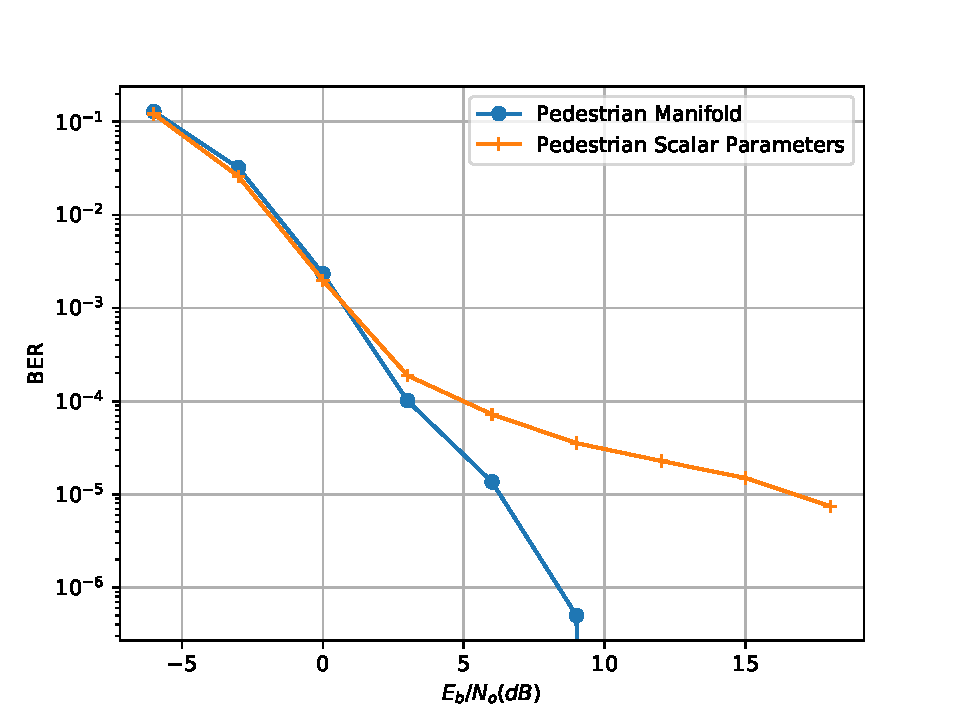
\includegraphics[width=0.5\textwidth]{images/pedestrian.pdf}

\caption{BER vs SNR for pedestrian channel}
\label{ber_overview}
\vspace{-5pt}
\end{figure}

\subsection{Performance Measurement}
\label{setting}

\noindent Since the Precoding matrices fundamentally lie on the Stiefel manifold, therefore, we are using the chordal distance parameter to measure the effectiveness of the quantization method used by us. Later we are comparing the ber rates with the ideal completely fed back subcarriers. Or simulations and discussions part 2 criteria could be used. Done similar work as in bhaskar rao paper but along with that we have tried to interpolate the joint interpolation in time and frequency at the transmitter. Also since we want to lower the number of bits we have used the method of interpolation and have achieved significant improvement over predictive quantization in the stiefel manifold paper which came in 2014 and also a variation which came in 2018 by Agrim gupta who tried to use joint interpolation of the stiefel manifold method. In fact we use joint interpolation of the scalar parameters which are easy to use gives better quantization than any of the above methods.
The advantage they had over the number of bits due to the 6 bit codebook they used is also achieved by us by using smart interpolation techniques, i.e. by dropping the feedback bits in alternating time instances as it is still going to follow the scalar parameters without much difference.
The problem of values hopping between pi and -pi is also tackled by wrapping the values around which we can show works nicely. The only drawback is that while initializing the parameter, they go out of their actual range and therefore using a uniform quantizer over the prescribed range does not work. But since most of the values lie between the given range we can use most of the initialization bits quantizing the parameters uniformly between the [-$\pi$ , $\pi$] and using smaller amount of bits between the range outside that which could go upto $-3\pi$ and $3\pi$, i.e. we are covering 300% more range outside the given area and that works mostly fine for the rest of the values.

Using the idea of joint interpolation given in the other paper.
\begin{figure}
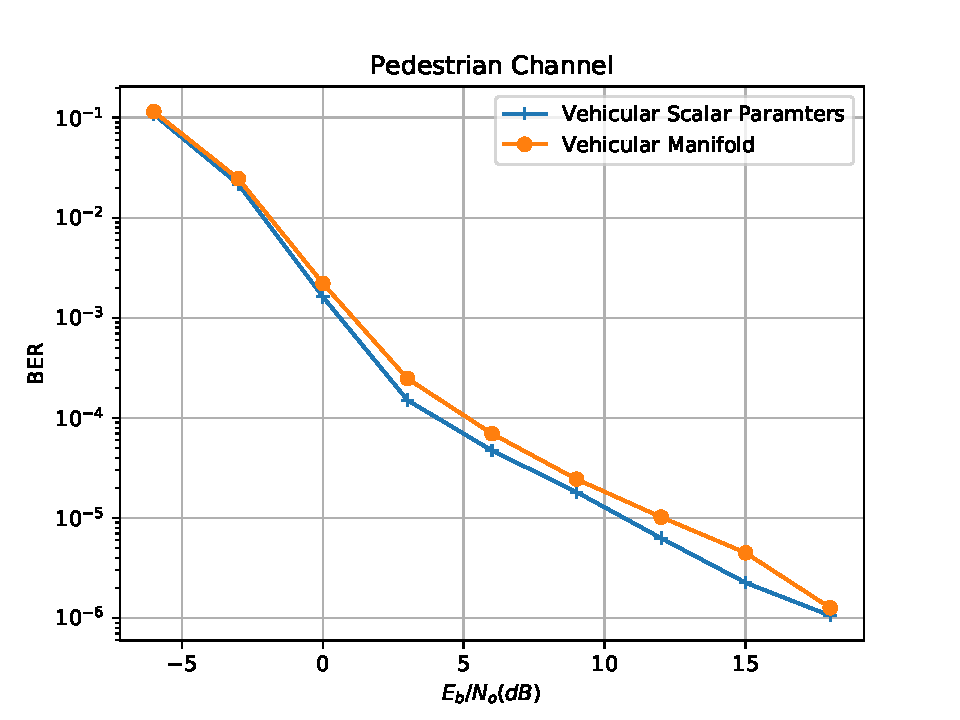
\includegraphics[width=0.5\textwidth]{images/vehicular_ber.pdf}

\caption{BER vehicular plot comparison between our method and agrims}
\label{ber_overview}
\vspace{-5pt}
\end{figure}

%Qtisn error with 1000 chan evols
%Qtisn error with 100 chan evols
%BER
%Achievable rat

\section{Conclusions and Future Work}
\label{section4}

We could reduce more by seeing the effect of sigma values(power distribution). We can save the bits by not sending for those which have very low sigma values. This could result in a very robust method.

\vspace{-4pt}

% \section{Acknowledgment}
% % \label {section6}
% % \input{sections/6_section.tex}
% Parts of this work was supported by the Bharti Centre for Communication in
% IIT Bombay, and the Visvesvaraya
% PhD Scheme of Ministry of Electronics \& Information Technology,
% Government of India, being implemented by Digital India Corporation.


\renewcommand{\bibfont}{\footnotesize}
\bibliography{IEEEabrv,main}
\bibliographystyle{IEEEtran}
\end{document}

% Remove the first para of FSM. State what r1,r2,d,\theta are in the FSM model states themselves. As a concluding statement of STAT-2 state that using the
% inherit geometery of the problem, we get AoA
